\documentclass[tikz]{standalone}
\usetikzlibrary{calc, intersections, math}

\begin{document}
	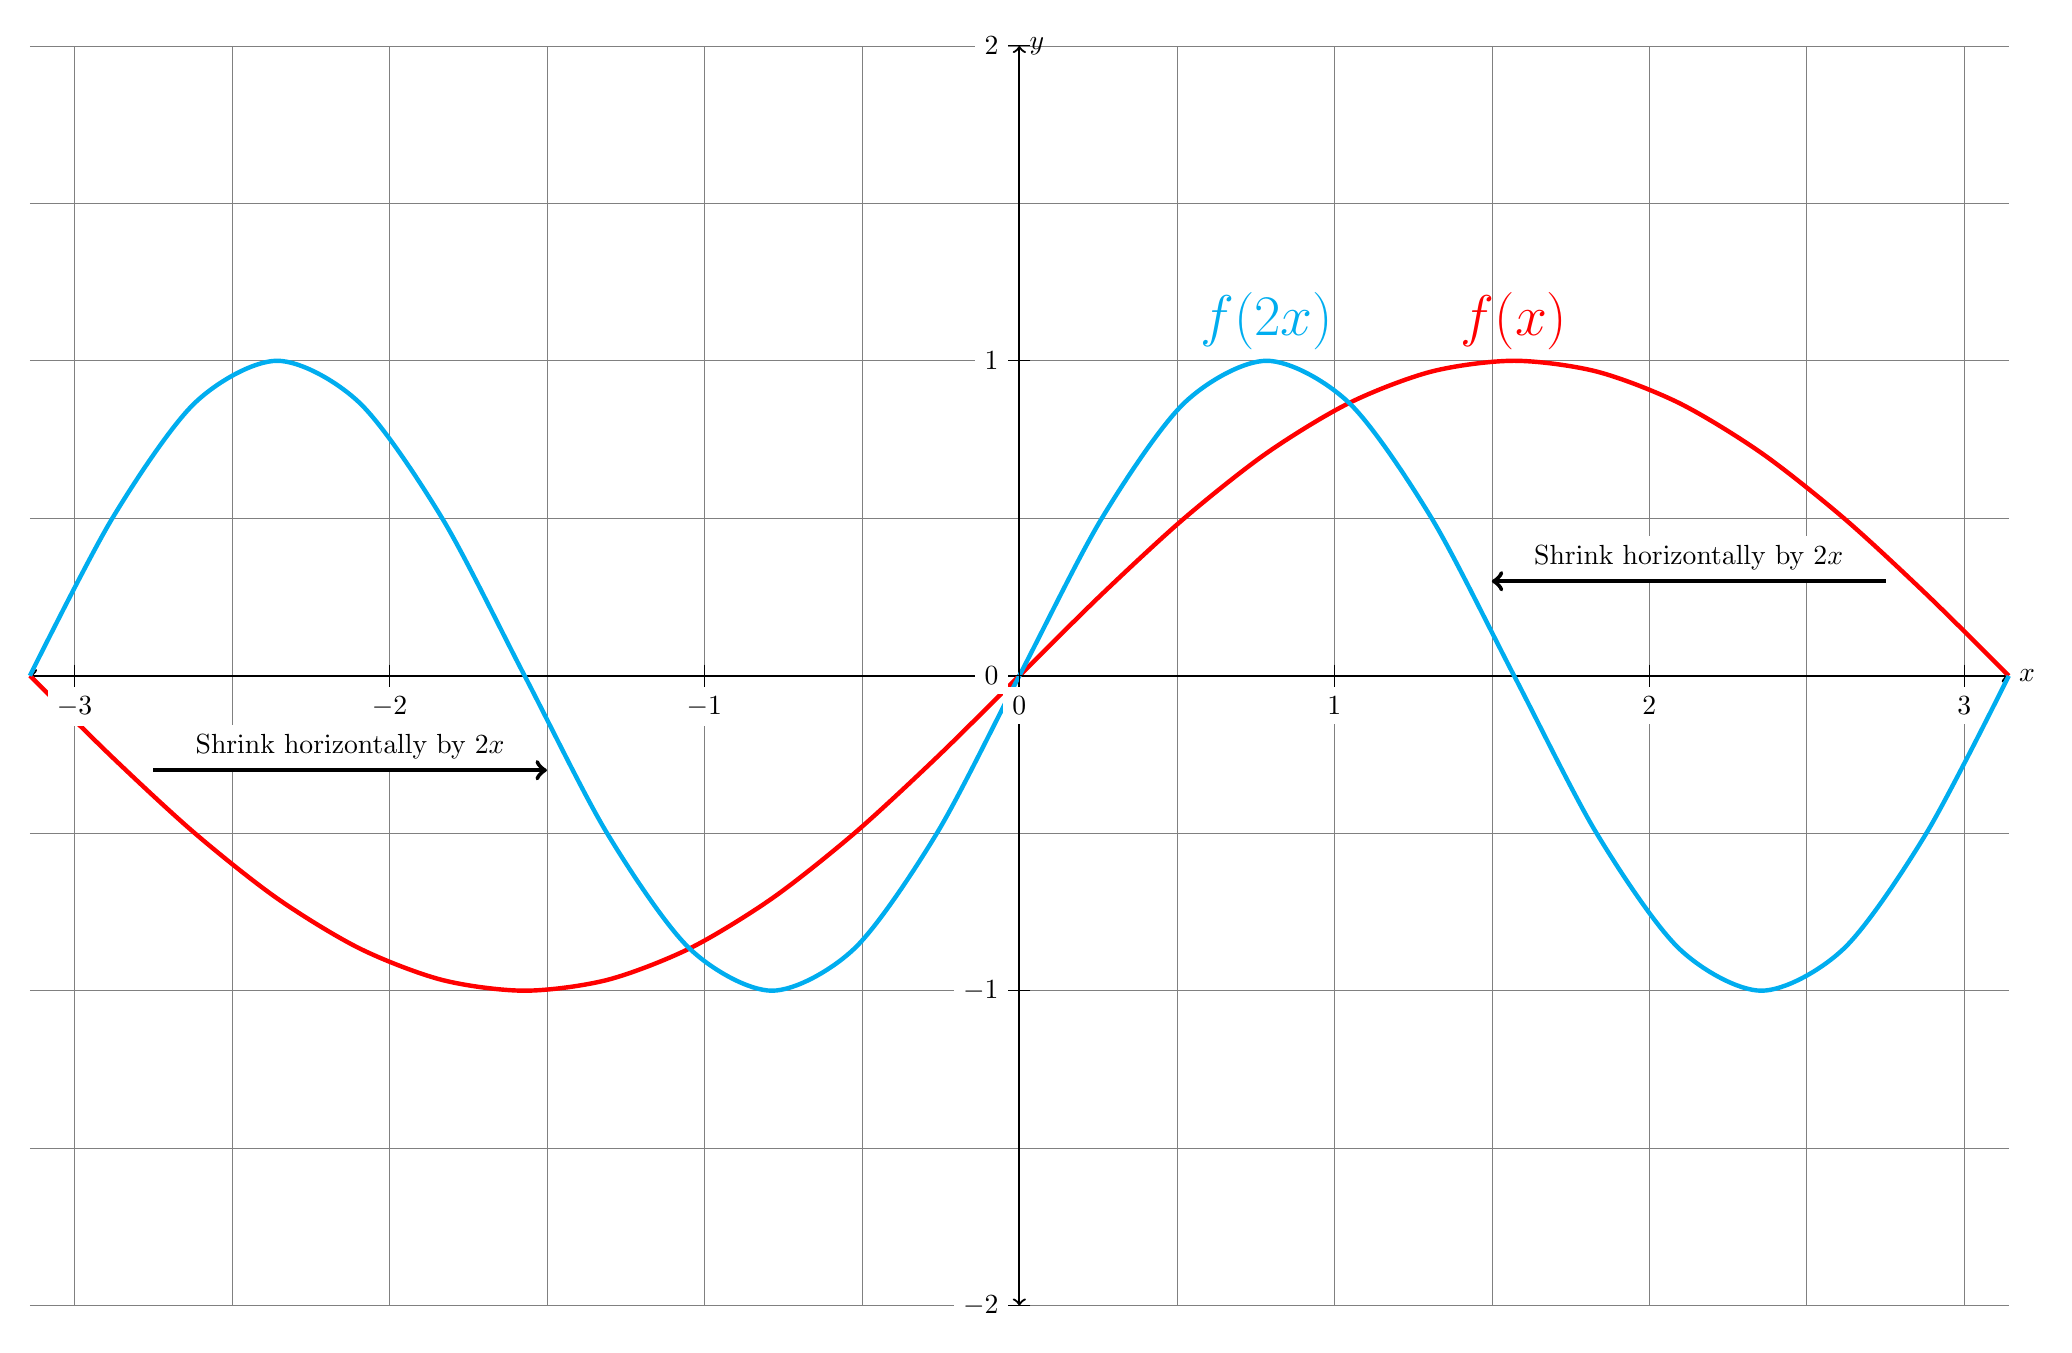
\begin{tikzpicture}[scale=4, mystyle/.style={circle,fill}]

		% set the window size. The \c notation allows us to use more complex variable names
		\tikzmath{\c{width} = pi;}

        % setting up the Cartesian Grid. Note "help lines" = "gray, very thin"
        \draw[step=.5cm,help lines] (-1*\c{width},-2) grid (\c{width},2);
        % setting up the real and imaginary axis. 
        \draw[thick, <->] (-1*\c{width},0) -- (\c{width},0) coordinate (x axis) node[right] {$x$};
        \draw[thick, <->] (0,-2) -- (0,2) coordinate (y axis) node[right] {$y$};;

	\draw[ultra thick,red,domain=-1*\c{width}:\c{width},smooth] plot (\x,{sin(\x r)});
	\node[ultra thick, red, above] at (pi/2,1) {\huge $f(x)$};


	\draw[ultra thick, ->] (2.75,.30) -- (1.5,.30) node[midway, above, fill=white] {Shrink horizontally by $2x$};
	\draw[ultra thick, ->] (-2.75,-.30) -- (-1.5,-.30) node[midway, above, fill=white] {Shrink horizontally by $2x$};

	\draw[ultra thick,cyan,domain=-1*\c{width}:\c{width},smooth] plot (\x,{sin(2*\x r)});
    \node[ultra thick, cyan, above] at (pi/4,1) {\huge $f(2x)$};

	\foreach \x in {-3,..., 3}
		\draw (\x cm,1pt) -- (\x cm,-1pt) node[anchor=north, fill=white] {$\x$};
 	\foreach \y in {-2,...,2}
		\draw (1pt,\y cm) -- (-1pt,\y cm) node[anchor=east, fill=white] {$\y$};

	\end{tikzpicture}


\end{document}
